\section{Research Design}\label{research-design}

This study employed computational simulation (\colorbox{yellow!40}{Law, 2015}) to explore
the integration of RL and TOC in addressing production scheduling within
stochastic manufacturing environments, along with the associated
practical and theoretical implications (\colorbox{yellow!40}{cf., Harrison et al. 2007;
Davis et al. 2007}). The research followed a structured five-stage
process, as illustrated in \colorbox{yellow!40}{\hyperref[_Ref187516847]{Figure 1}}: (i)
construction of the virtual environment; (ii) development of the
simulation model based on the TOC solution; (iii) creation of the
simulation model integrating RL and TOC; (iv) execution of simulation
experiments; and (v) summative and formative evaluation.

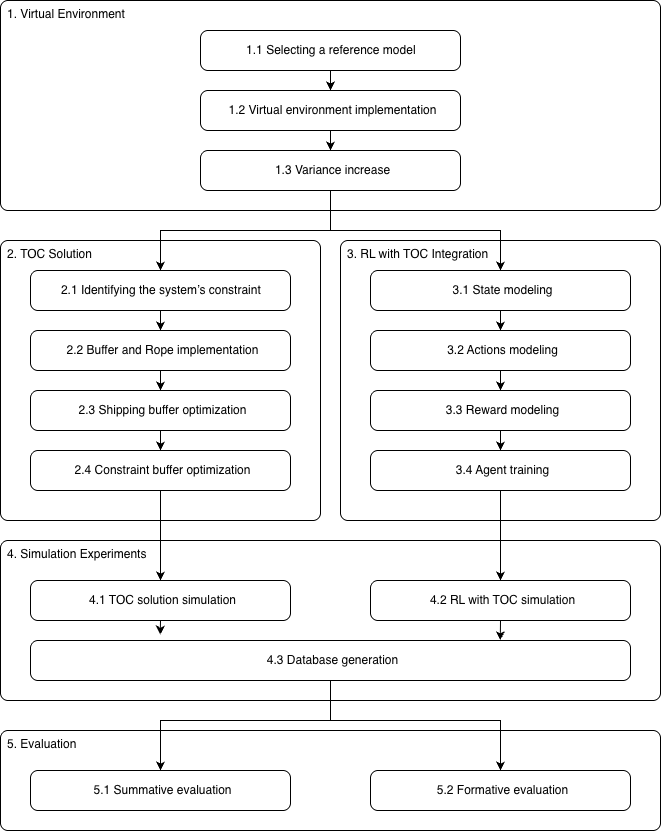
\includegraphics[width=4.08151in,height=5.13122in]{figures/fig01.png}

\protect\phantomsection\label{_Ref187516847}{}\colorbox{yellow!40}{Figure 1.}
\colorbox{yellow!40}{Overview of the research design.}

In stage 1, the virtual environment was constructed as the foundation
for creating the two subsequent simulation models in stages 2 and 3. The
process began with selecting a reference model in step 1.1. The
discrete-event simulation model proposed by (Atwater and Chakravorty,
2002a) was chosen for its ability to simulate a stochastic manufacturing
environment with multiple products, resources, and production routes
(see \colorbox{yellow!40}{\hyperref[_Ref187516873]{Figure 2}}). In step 1.2, we used this
reference model to implement the virtual environment computationally,
employing Python along with the SimPy framework for discrete-event
simulation (\colorbox{yellow!40}{Reference}) and OpenAI Gym, a toolkit for developing and
comparing RL algorithms (\colorbox{yellow!40}{Reference}). Finally, in step 1.3, we
introduced additional probabilistic elements to the validated model to
increase the variance of the virtual environment (\colorbox{yellow!40}{cf., Machado et
al., 2023}). These elements included resource changeovers and downtime,
such as time between failures and time to repair.

In stage 2, the virtual environment was used to develop a simulation
model that incorporated a TOC-based scheduling solution, combining DBR
and BM. First, an operational assessment of the virtual environment was
conducted, which led to identifying the system's constraint in step 2.1.
In step 2.2, once the constraint (i.e., the drum) was defined, the
remaining two elements of DBR --- the buffer and the rope --- were
implemented following (Schragenheim, 2010c). Two types of buffers were
considered (see \colorbox{yellow!40}{\hyperref[_Ref187516903]{Figure 3}}): (i) the CB and
(ii) the SB. The rope was implemented as a logic for creating,
scheduling, and releasing orders and raw materials at the system's
entrance, based on the consumption of both buffers. A BM policy was then
introduced and applied to optimize the reference levels of the shipping
buffers in steps 2.3 (Schragenheim, 2010c). In step 2.4, an experiment
was conducted to identify the best reference level for CB.

As in stage 2, the virtual environment informed the development of the
simulation model that integrated RL and TOC into a production scheduling
solution in stage 3. In step 3.1, fifty-two state variables were
considered, capturing the current quantity of each product being
processed throughout the system, including in the CB and SB. With
respect to the agent's actions, in step 3.2 we the decisions as how much
of each product to produce during the replenishment interval. The
scheduling and release of orders followed the logic established by TOC
(see \colorbox{yellow!40}{\hyperref[_Ref187516938]{Figure 5}}). In step 3.3, the reward
function was modeled by incorporating four penalty subfunctions aligned
with TOC's two key performance measures: (i) throughput and (ii)
inventory. Finally, in step 3.4, the PPO algorithm was employed to train
the agent in its search for the optimal policy (\colorbox{yellow!40}{cf. Reference}).
This training process was carried out across 100,000 interactions and
implemented using the Stable Baselines3 library (\colorbox{yellow!40}{Raffin et al.,
2021}).

In stage 4, both simulation models --- one based on TOC (step 4.1) and
the other integrating RL with TOC (step 4.2) --- were executed over
multiple replications (or episodes), simulating 200.000 time units of
operation. The performance measures used as model outputs included: (i)
the number of products produced and sold; (ii) the average number of
parts in process; (iii) the average lead-time; and (iv) the average
inventory, all measured over a predefined replenishment interval. In
step 4.3, these measures were recorded both by individual product and in
aggregate, resulting in a database generated from the simulation runs.

In the final stage, the database of simulation runs underwent both
summative and formative evaluations (\colorbox{yellow!40}{cf., Venable, 2016}). The
summative evaluation (step 5.1) aimed to quantify the performance
difference between the two simulation models, using the TOC-based model
as a reference. This analysis employed a confidence interval for the
paired mean difference (\colorbox{yellow!40}{cf., Law, 2015 p. 560}). The formative
evaluation (step 5.2) focused on understanding and explaining the
underlying reasons for the observed performance differences. This
process unfolded in two phases. First, three analytical techniques were
applied --- Spearman's coefficient (\colorbox{yellow!40}{Yu et al., 2021}), multiple
linear regression (\colorbox{yellow!40}{Nathans et al., 2012}), and decision trees
(\colorbox{yellow!40}{Kuhnle et al., 2022}) --- to explore the relationship between state
variables and the actions taken in each model. Based on the insights
drawn from these analyses, mechanism-based explanations were formulated
to articulate the dynamic hypotheses underlying the key differences
(\colorbox{yellow!40}{cf., Gauss et al. 2024a}). This also highlighted opportunities for
improving traditional DBR. Finally, in step 4.3, a new TOC-based
simulation model incorporating the modified DBR approach was built and
again compared with the model integrating RL and TOC. Further details
about the virtual environment and simulation models are provided in
section 4, while sections 5 and 6 present the simulation runs and the
summative and formative evaluations, respectively.
